\subsection{\texorpdfstring{Ромбовидное свойство и параллельная редукция}{Diamond property and parallel reduction}}

\begin{definition}[ромбовидное свойство]
    $G$ обладает ромбовидным свойством, если какие бы ни были $a$, $b$, $c$, что $aGb$, $aGc$, $b \ne c$, найдётся такое $d$, что $bGd$ и $cGd$.
\end{definition}

\begin{example}
    $(<)$ на натуральных числах обладает ромбовидным свойством.
    $(>)$ на натуральных числах не обладает ромбовидным свойством.
\end{example}

$\beta$-редукция не обладает ромбовидным свойством.
\usetikzlibrary{arrows.meta}
\begin{figure}[h]
    \centering
    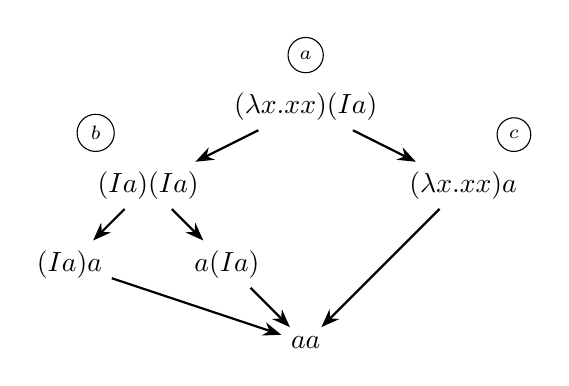
\begin{tikzpicture}[->,>={Stealth[black]},
                every edge/.style={draw=black,thick}]
        \node[label={\scriptsize\tikz\node[circle,draw]{$a$};}]     at (0,   0) (A)  {$(\lambda x . x x)(\comb Ia)$};
        \node[label={135:\scriptsize\tikz\node[circle,draw]{$b$};}] at (-2, -1) (B)  {$(\comb Ia)(\comb Ia)$};
        \node[label={45:\scriptsize\tikz\node[circle,draw]{$c$};}]  at (2,  -1) (C)  {$(\lambda x . x x) a$};
        \node                                                       at (-3, -2) (B1) {$(\comb Ia)a$};
        \node                                                       at (-1, -2) (B2) {$a(\comb Ia)$};
        \node                                                       at (0,  -3) (D)  {$aa$};

        \path (A)  edge (B)
                   edge (C)
              (B)  edge (B1)
                   edge (B2)
              (B1) edge (D)
              (B2) edge (D)
              (C)  edge (D);
    \end{tikzpicture}
    \captionsetup{labelformat=empty}
    \caption{Нет такого $d$, что $b \rightarrow_{\beta} d$ и $c \rightarrow_{\beta} d$.}
\end{figure}

\begin{theorem}[Чёрча-Россера] \label{church-rosser}
    $\beta$-редуцируемость обладает ромбовидным свойством.
\end{theorem}

\begin{lemma}
    Если $R$ обладает ромбовидным свойством, то $R^{*}$ обладает ромбовидным свойством.
\end{lemma}

\begin{proof}
    Пусть $M_1 R^* M_n$ и $M_1 R N_1$. Тогда существуют такие $M_2 \ldots M_{n-1}$, что $M_1 R M_2$ \ldots $M_{n-1} R M_n$.
    Так как $R$ обладает ромбовидным свойством, $M_1 R M_2$ и $M_1 R N_1$, то существует такое $N_2$,
    что $N_1 R N_2$ и $M_2 R N_2$. Аналогично, существуют такие $N_3 \ldots N_n$, что $N_{i-1} R N_{i}$ и $M_i R N_i$.
    Мы получили такое $N_n$, что $N_1 R^* N_n$ и $M_n R^* N_n$.

    Пусть теперь $M_{1,1}R^*M_{1,n}$ и $M_{1,1}R^*M_{m,1}$, то есть имеются $M_{1,2}$\ldots$M_{1,n-1}$ и $M_{2,1}$\ldots$M_{m-1,1}$,
    что $M_{1,i-1} R M_{1,i}$ и $M_{i-1, 1} R M_{i, 1}$.
    Тогда существует такое $M_{2,n}$, что $M_{2,1} R^* M_{2,n}$ и $M_{1,n} R^* M_{2,n}$.
    Аналогично, существуют такие $M_{3,n}\ldots M_{m,n}$, что $M_{i,1} R^* M_{i,n}$ и $M_{1,n} R^* M_{i,n}$.
    Тогда $M_{1,n} R^* M_{m,n}$ и $M_{m,1} R^* M_{m,n}$.
\end{proof}

\begin{definition}[Параллельная $\beta$-редукция]
    $A \rightrightarrows_{\beta} B$
    \begin{enumerate}
        \item Если $A =_\alpha B$, то $A \rightrightarrows_{\beta}B$
        \item Если $A \rightrightarrows_{\beta} B$, то $\lambda x.A \rightrightarrows_{\beta} \lambda x . B$
        \item Если $P \rightrightarrows_{\beta} Q$ и $R \rightrightarrows_{\beta} S$, то $PR \rightrightarrows_{\beta} QS$
        \item Если $P \rightrightarrows_{\beta}R$ и $Q \rightrightarrows_{\beta} S$,
            то $(\lambda x . P) Q \rightrightarrows_{\beta} R_{[x\coloneqq{}S]}$.
    \end{enumerate}
\end{definition}

\begin{statement} \label{st-star}
    $(\rightrightarrows_{\beta})$ обладает ромбовидным свойством.
\end{statement}

\begin{proof}
    \todo % TODO
\end{proof}

\begin{statement} \label{st-A}
    Если $A \rightarrow_{\beta} B$, то $A \rightrightarrows_{\beta} B$.
\end{statement}

\begin{statement} \label{st-B}
    Если $A \rightrightarrows_{\beta} B$, то $A \twoheadrightarrow_{\beta} B$.
\end{statement}

\begin{proof}
    \todo % TODO
\end{proof}

При этом, обратное не всегда верно.
\begin{gather*}
    (\lambda x . x x) (\lambda x . x x x) \twoheadrightarrow_{\beta} (\lambda x . x x x)(\lambda x . x x x)(\lambda x . x x x) \\
    (\lambda x . x x) (\lambda x . x x x) \cancel{\rightrightarrows_{\beta}} (\lambda x . x x x)(\lambda x . x x x)(\lambda x . x x x)
\end{gather*}

\begin{statement} \label{st-C}
    Из \ref{st-A} и \ref{st-B} следует, что $(\rightarrow_{\beta})^{*} = (\rightrightarrows_{\beta})^{*}$.
\end{statement}

\begin{proof}
    Теорема \nameref{church-rosser} следует из \ref{st-star} и \ref{st-C}.
\end{proof}

\begin{corollary}
    Нормальная форма для $\lambda$-выражения единственна, если существует.
\end{corollary}

\begin{theorem}[Тезис Чёрча]
    Если функция вычислима с помощью механического аппарата, то она вычислима с помощью $\lambda$-выражения.
\end{theorem}

\subsection{\texorpdfstring{Порядок редукции}{Order of reduction}}
\epigraph{"<Завтра! Завтра! Не сегодня!"> "--- так ленивцы говорят.}{Das deutsches Sprichwort}

\begin{definition}
\[
    \comb K = \lambda x \lambda y . x \qquad
    \comb I = \lambda x . x \qquad
    \comb S = \lambda x y z . x z (y z)
\]
\end{definition}
$\comb I$ выражается через $\comb S$ и $\comb K$: $\comb I = \comb S \comb K \comb K$.

\begin{statement} \label{SK-basis}
    Пусть $A$ "--- замкнутое $\lambda$-выражение.
    Тогда найдётся выражение $T$, состоящее только из $\comb S$ и $\comb K$, что $A =_{\beta}T$.
\end{statement}

\begin{example}
    тут какой-то пример с омегой, подскажите чё там было, \todo % TODO
\end{example}

\begin{definition}[Нормальный порядок редукции]
    Нормальным порядком редукции называется редукция самого левого $\beta$-редекса.
\end{definition}
"<Ленивые вычисления"> (ну, почти, в ленивых ещё есть меморизация)

\begin{definition}[Аппликативный порядок редукции]
    Самый левый из самых вложенных.
\end{definition}
"<Энергичные вычисления">

\begin{statement}
    Если нормальная форма существует, она может быть достигнута нормальным порядком редукции.
\end{statement}

\subsection{\texorpdfstring{Парадокс Карри}{Curry's paradox}}

Попробуем построить логику на основе $\lambda$-исчисления.
Введём комбнатор-импликацию, обозначим $(\supset)$. Введём M.P. и правила:
\begin{enumerate}
    \item $A \supset A$
    \item $(A \supset (A \supset B)) \supset (A \supset B)$
    \item $A =_{\beta} B$, тогда $A \supset B$
\end{enumerate}

Покажем, как в полученной логике можно доказать любое утверждение.
Введём обозначение: $Y_{\supset a} \equiv Y (\lambda t . t \supset a) =_{\beta} Y (\lambda t . t \supset a) \supset a$.

\begin{tabular}{lll}
    1) & $Y_{\supset a} \supset Y_{\supset a}$ & (схема аксиом) \\
    2) & $Y_{\supset a} \supset (Y_{\supset a} \supset a)$ & (можно доказать) \\
    3) & $(Y_{\supset a} \supset Y_{\supset a} \supset a) \supset (Y_{\supset a} \supset a)$ & (схема аксиом) \\
    4) & $Y_{\supset a} \supset a$ & (M.P.) \\
    5) & $(Y_{\supset a} \supset a) \supset Y_{\supset a}$ & (третье правило) \\
    6) & $Y_{\supset a}$ & (M.P.) \\
    7) & $a$ & (M.P.)
\end{tabular}

Получается, что данная логика противоречива. Показать это нам дал возможность тот факт,
что в нашей логике с помощью $Y$-комбинатора мы можем ссылаться в утверждении на само себя.
Аналогично можно прийти к парадоксальному выводу из высказывания "<если это утверждение верно, то русалки существуют"> на нашем мета-языке.

\subsection{\texorpdfstring{Импликационный фрагмент ИИВ}{Implication fragment of intuitionistic logic}}

\begin{definition}[импликационный фрагмент ИИВ]
    Рассмотрим интуиционистское исчисление высказываний.
    \begin{enumerate}
        \item Введём схему аксиом:
        \[
            \infer{\Gamma, \varphi \vdash \varphi}{}
        \]
        \item Правило введения импликации:
        \[
            \infer{\Gamma \vdash \varphi \rightarrow \psi}{\Gamma, \varphi \vdash \psi}
        \]
        \item И правило удаления импликации:
        \[
            \infer{\Gamma \vdash \psi}{\Gamma \vdash \varphi \rightarrow \psi && \Gamma \vdash \varphi}
        \]
    \end{enumerate}

    Мы построили импликационный фрагмент ИИВ (и.ф.и.и.в).
\end{definition}

\begin{example} Докажем $\varphi \rightarrow \psi \rightarrow \varphi$:
\[
    \infer[(2)]
        { \vdash \varphi \rightarrow (\psi \rightarrow \varphi) }
        { \infer[(2)]
            { \varphi \vdash \psi \rightarrow \varphi }
            { \infer[(1)]
                { \varphi, \psi \vdash \varphi}
                {}
            }
        }
\]
\end{example}

\begin{theorem}
    И.ф.и.и.в полон в моделях Крипке, то есть $\Gamma \vdash \varphi$ т.и.т.т.,
    когда для любой модели крипке $C$ из $\Vdash_C \Gamma$ следует $\Vdash_C \varphi$.
\end{theorem}

\begin{proof}
    Рассмотрим модель Крипке вида $W = \left\{\Delta \mid \Gamma \subseteq \Delta, \Delta\text{ замкнуто относительно }\vdash\right\}$,
    $\Gamma \leq \Delta$ если $\Gamma \subseteq \Delta$.
    Индукцией по структуре $\varphi$ покажем, что $\Delta \Vdash \varphi$ т.и.т.т., когда $\Delta \vdash \varphi$:
    \begin{enumerate}
        \item Пусть $\varphi \equiv x$ "--- переменная. Тогда $\Gamma \vdash \varphi$ эквивалентно $x \in \Gamma$, что эквивалентно $\Vdash x$ (по определению).
        \item Пусть $\varphi \equiv \alpha \rightarrow \beta$.
        \begin{enumerate}[label=(\asbuk*)]
            \item Пусть $\Delta \vdash \varphi$.
            Рассмотрим такое $\Delta'$, что $\Delta \leq \Delta'$ и $\Delta' \Vdash \alpha$.
        \end{enumerate}
        ой всё \todo
    \end{enumerate}
\end{proof}

\begin{corollary}
    И.ф.и.и.в замкнут относительно выводимости.
\end{corollary}
Если некоторое утверждение выводится в ИИВ ($\vdash_{и} \varphi$) и содержит только импликации,
то оно выводится и в и.ф.и.и.в. ($\vdash_{и \rightarrow} \varphi$).
